\section{Benutzer Client}

	\subsection{UML2-Komponentendiagramm}
		\begin{center}
			\begin{figure}[H]
    		\centering
    		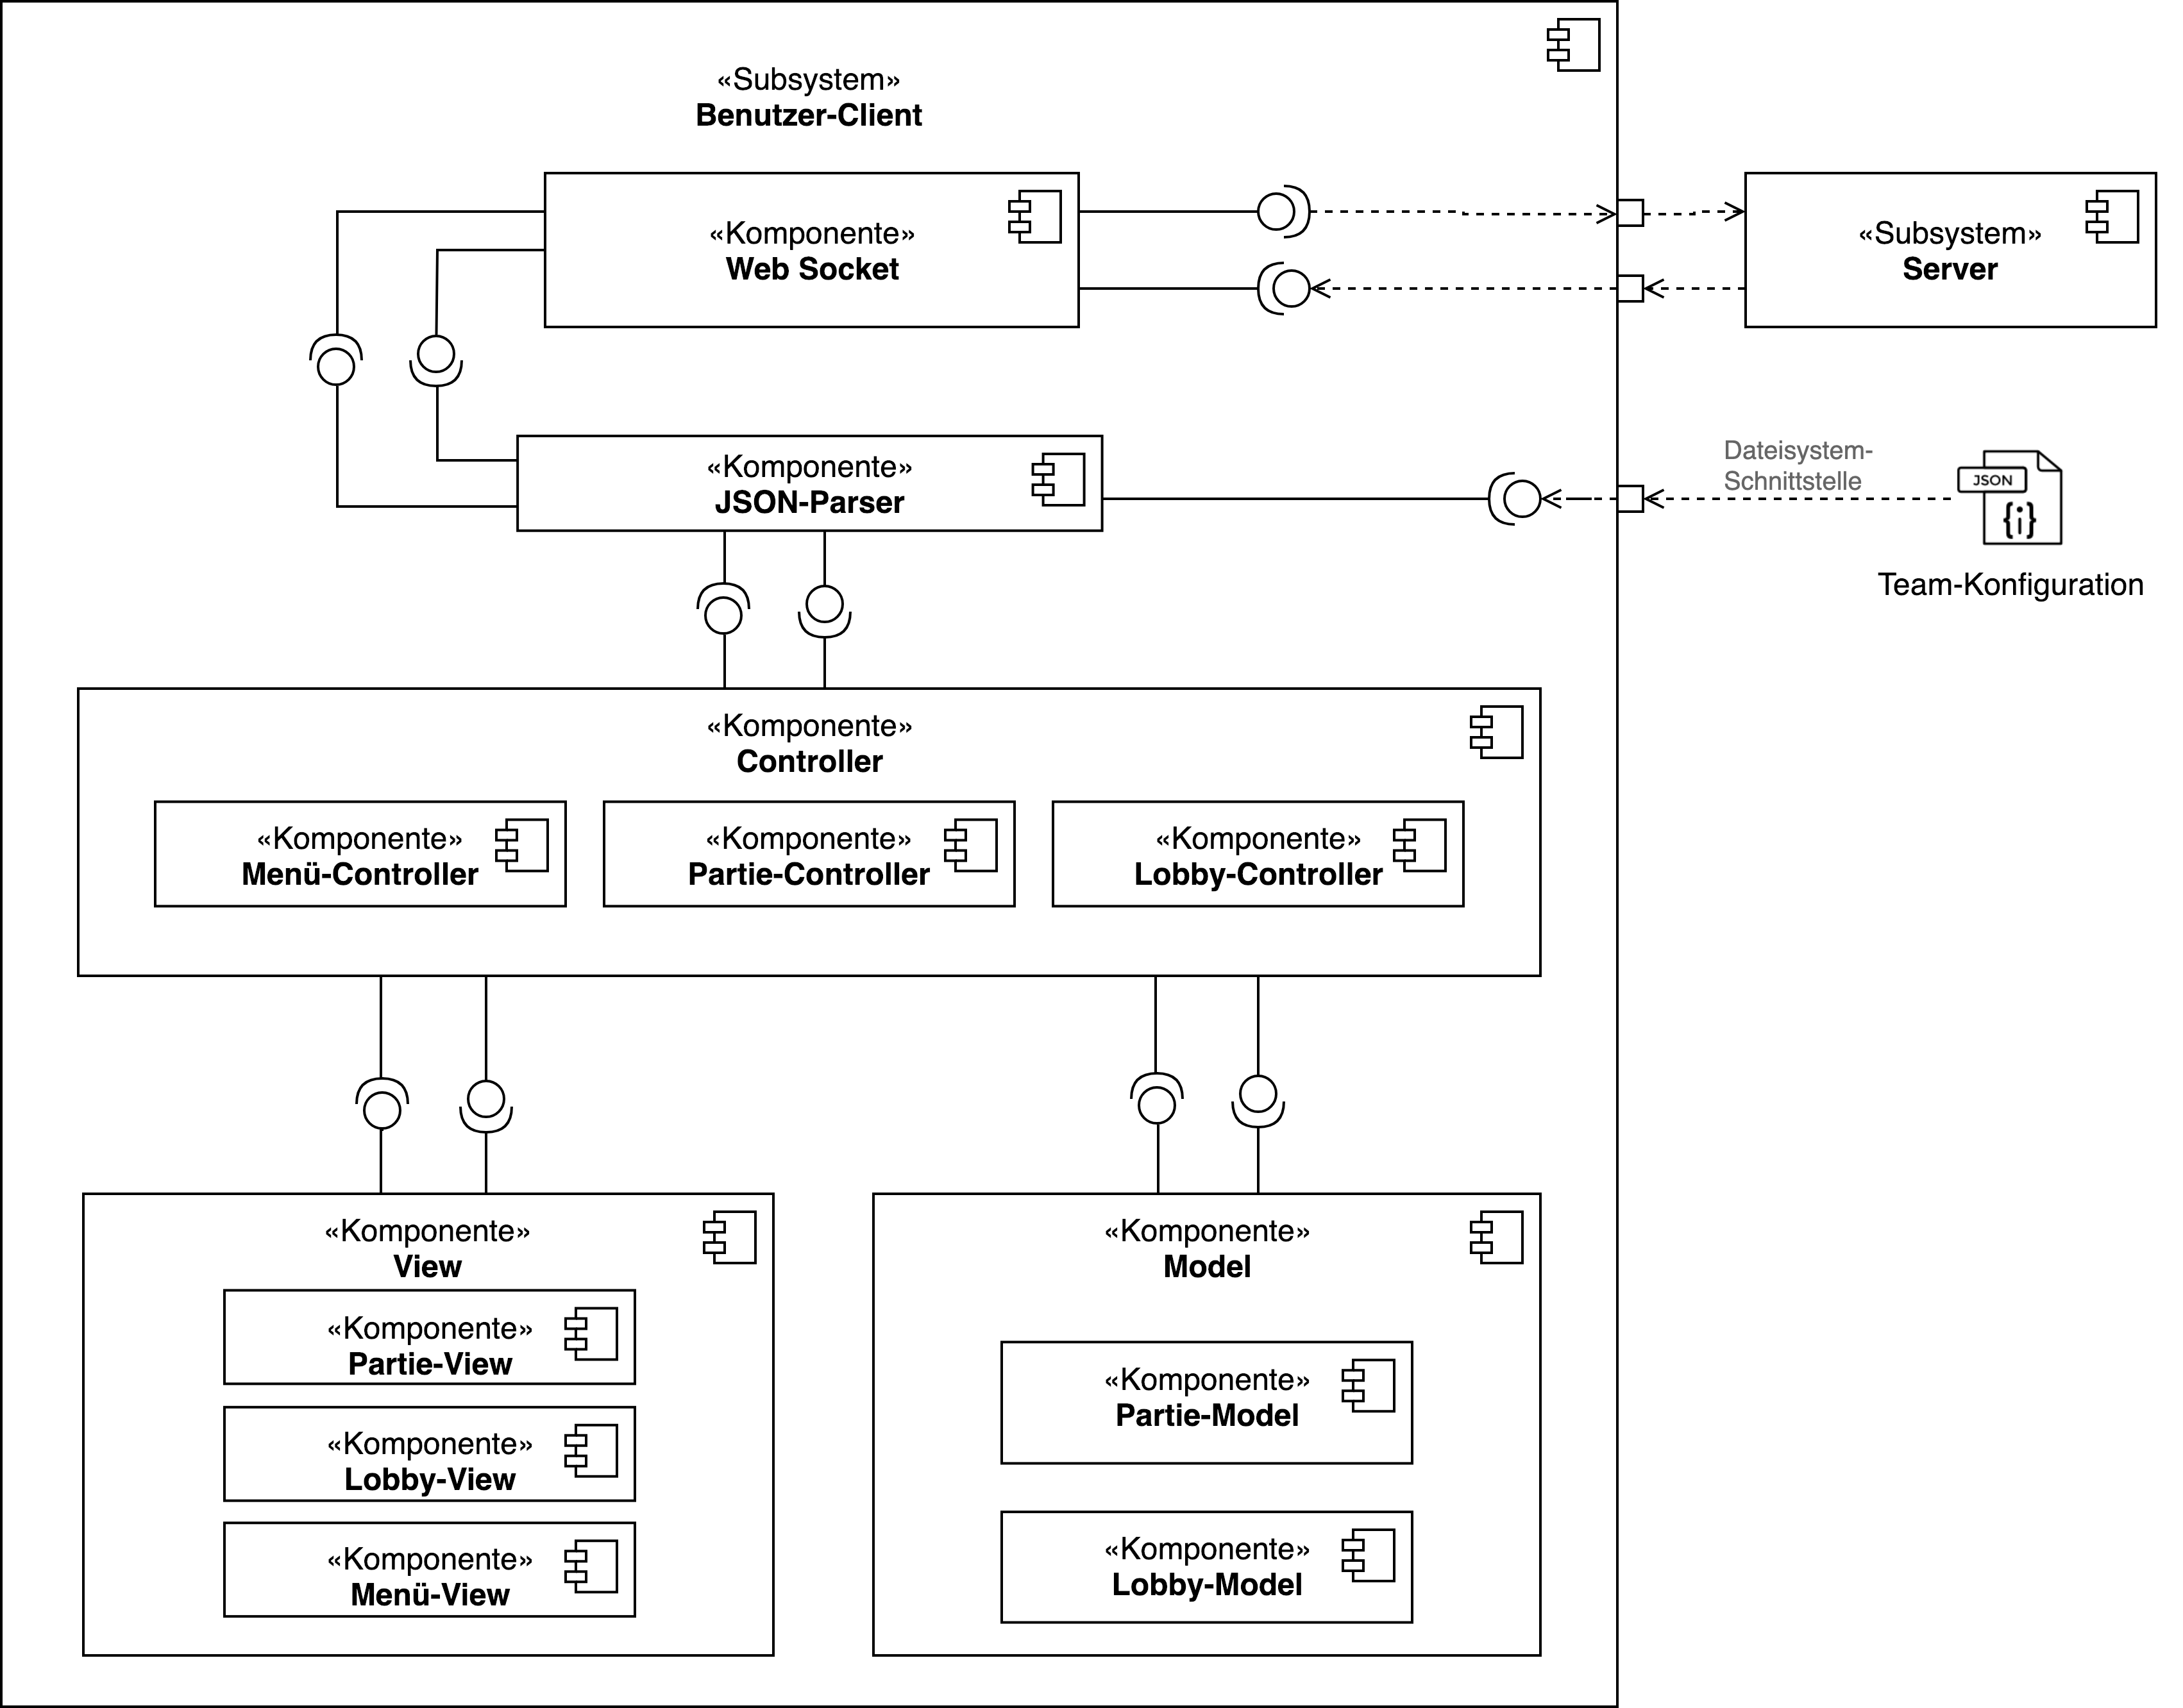
\includegraphics[scale=0.13]{images/komponentendiagramm_benutzer-client.png}
		\end{figure}
		\end{center}
		

	\subsection{Beschreibungen}

		\begin{description}
			\item[Benutzer-Client]
			Beim Benutzer-Client handelt es sich um eine Anwendung mit grafischer Benutzeroberfläche mit der \textit{Fantastic Feasts}-Partien beigetreten werden kann und diese auf verschiedene Weisen verfolgt werden können. In einer Lobby können Partien auf einem Server erstellt werden oder es kann einer bestehenden Partie auf einem Server beigetreten werden. Die Spiellogik einer Partie läuft jedoch auf dem Server. Eine Partie lässt sich sowohl passiv als Beobachter verfolgen als auch aktiv als Spieler gestalten. In diesem Fall nimmt der Benutzer-Client Spieleraktionen entgegen und sendet sie an den Server.
			Es wird eine Model-View-Controller-Architektur gewählt, da sowohl vom Server als auch vom Benutzer Eingaben erfolgen können. Das Behandeln dieser Eingaben wird zentral vom Controller übernommen, sodass beispielsweise das Umsetzen der Nutzereingaben nicht an die View gekoppelt ist. Das würde dazu führen, dass sich die View, also die reine Darstellung, nur schwer unabhängig von der Logik verändern ließe. Ein Model ist notwendig, um die Spielzustände auf dem Benutzer-Client eindeutig zu verwalten. Somit können beispielsweise vorab Einschränkungen auf erlaubte Spielzüge vorgenommen werden, ein Zug auf Vollständigkeit geprüft und die Darstellungen der View am Model orientiert werden. Das Model wird allerdings nicht die gesamte Spiellogik enthalten, da dies Aufgabe des Servers ist.
			
			\item[Controller]
			Der Controller ist die Schaltstelle aller Aktionen im Benutzer-Client. Er besteht aus den drei Komponenten Menü-Controller, Spiel-Controller und Lobby-Controller.		
			
			\begin{description}
				\item[Menü-Controller]
				Der Menü-Controller beinhaltet die Logik, mit der im Menü zwischen verschiedenen Ansichten hin und her gewechselt werden kann. Über ihn kann das Spiel beendet werden, die Lobby betreten, zur Hilf-Ansicht gewechselt werden oder etwaige Einstellungen am Benutzer-Client vorgenommen werden. Er updatet die Menu-View und behandelt Nutzereingaben entsprechend. 
				
				\item[Spiel-Controller]
				Der Spiel-Controller hat zwei Aufgaben. Einerseits behandelt er alle Ereignisse und Nutzereingaben, die über die Spiel-View bereitgestellt werden und leitet sie an das Model bzw. den Server weiter. Andererseits nimmt er Spieldaten vom Server bzw. dem JSON-Parser entgegen und aktualisiert damit die Partie-View und das Partie-Model des Benutzer-Clients. Er sorgt dafür, dass die View nur Nutzereingaben zulässt, die erlaubt sind. Diese Information erhält er vom Model.
				
				\item[Lobby-Controller]
				Mit dem Lobby-Controller werden die Interaktionen in der Lobby zwischen Server, Benutzer-Client-Anwendung und Nutzereingaben behandelt. Insbesondere kann über den Lobyy-Controller mithilfe des JSON-Parsers eine Schnittstelle zum Dateisystem hergestellt werden, wodurch eine Team-Konfiguration ausgewählt werden kann.
			\end{description}
			
			\item[View]
			Die View enthält alle Klassen, die die grafische Benutzeroberfläche des Benutzer-Clients bilden. Sie unterteilt sich in die drei Komponenten Menü-View, Lobby-View und Partie-View.
			\begin{description}
				\item[Partie-View]
				Die Partie-View enthält alle Klassen, die die grafische Darstellung einer Partie sowohl im Beobachter- als auch im Spieler-Modus ausmachen. Nutzereingaben und Ereignisse werden an den entsprechenden Controller weitergeleitet.
			
			
				\item[Lobby-View]
				Die Lobby-View enthält alle Klassen, die zur grafischen Darstellung der Partie-Lobby notwendig sind. Nutzereingaben werden an den entsprechenden Controller weitergeleitet.
			
			
				\item[Menü-View]
				Die Menü-View enthält alle Klassen, die zur grafischen Darstellung des Menüs notwendig sind. Nutzereingaben werden an den entsprechenden Controller weitergeleitet.

			\end{description}
			
			
			
			\item[Model]
			Das Model ist eine Gruppe von Klassen, die wichtige Zustände des Benutzer-Clients repräsentieren und Zustandsübergänge festlegen.
			
			\begin{description}
				\item[Lobby-Model]
				Das Lobby-Model fasst die Klassen zusammen, die die Zustände der Lobby repräsentieren. Dazu gehören zum Beispiel vorhandene Partien und beigetretene Spieler bzw. Beobachter. Auch bestehende Verbindungen mit dem Server werden hier repräsentiert.
			
				\item[Partie-Model]
				Das Partie-Modell ist eine stark vereinfachte Variante der Spiellogik auf dem Server. Sie beschränkt sich darauf, einen Partie-Zustand eindeutig zu beschreiben und die Regeln für erlaubte Spielzüge zu kennen. So wird ermöglicht, dass der Spieler nur erlaubte Züge durchführen kann und diese Information nicht jedes mal vom Server angefordert werden muss. Zusätzlich hilft das Model dabei, eine konsistente Darstellung der Partie zu erhalten, da die View sich stets an den Zuständen des Models orientiert.
			\end{description}
			
			\item[Kommunikator]
			Der Kommunikator de bildet die Komponente, die sich um die Datenübertragung mit dem Server kümmert. Daten über den Spielzustand werden vom Server empfangen und Spieleraktionen werden an den Server gesendet.
			
			\item[JSON-Parser]
			Der JSON-Parser wandelt die JSON-Daten in interne Objekte der Software um und umgekehrt. Da auch in den Client-Anwendungen eine ähnliche Komponente von Nöten ist, bietet es sich an diese Funktionalitäten in einer eigenen Komponente auszulagern.  

		\end{description}
		
	\subsection{Zuordnung der Funktionalen Anforderungen}
	
	Die funktionalen Anforderungen gemäß dem Pflichtenheft werden den Komponenten folgendermaßen zugeteilt:
	
	\begin{center}
		\begin{tabular}{|l|l|}
			\hline
			\textbf{Komponente} & \textbf{Abgedeckte funktionale Anforderungen}\\ \hline
			Menü-Controller & FA56 \\ 
			& FA60 \\
			& FA65 \\
			& FA67 \\ \hline
		
			Lobby-Controller & FA61 \\
			& FA56 \\
			& FA63 \\
			& FA67 \\ \hline
		
			Partie-Controller & FA56 \\
			&  FA67-69 \\
		
			Menü-View & FA56 \\ 
			& FA60 \\
			& FA65 \\ \hline
		
			Lobby-View & FA61 \\ 
			& FA63 \\ \hline
		
			Partie-View & FA62 \\ 
			& FA64 \\ 
			& FA66 \\ \hline
		
			Partie-Model & FA01-52 \\ 
			& FA60 \\
			& FA65 \\ \hline
		
			Lobby-Model & FA61 \\ 
			& FA63 \\
			& FA65 \\ \hline
		
			Web Socket & FA55 \\ \hline
		
			JSON-Konverter & FA53 \\
			& FA57\\ \hline
		\end{tabular}	
	\end{center}
	